\section{$\varepsilon$-сети и вполне ограниченность. Свойства. Связь с компактностью. Теорема о характеристике компактов в $\R^d$}

\begin{conj}
    $(X, \rho)$ --- метрическое пространство. $A \subset X$ --- множество.

    $E \subset A$ --- $\varepsilon$-сеть для $A$, если $\forall a \in A$ найдётся $e \in E$, т.ч. $\rho(a, e) < \varepsilon$

    то есть $A \subset \bigcup\limits_{e \in E} B_{\varepsilon}(e)$.

\end{conj}

\textbf{Комментарий:}
В чём смысл этой штуки?
Вот у нас есть какое-то пространство, допустим $R^3$.
И вы хотите описать как-то множество в этом пространстве,
описать с некоторой точностью, запихать в компьютер описание множества.
Понятно, что совсем абстрактное множество вы не сумеете запихать в компьютер,
и поэтому можно это сделать с некоторой точностью,
с точностью до какого-то $\varepsilon$. 

Как это сделать? Нужно взять некоторый набор точек,
такой что для каждого элемента из множества $A$ у нас будет представитель, который
отличается от $a$-маленького не больше чем на $\varepsilon$.

Таким образом мы запихаем не множество $A$, а некоторое множество, которое его побольше, но такое что с точностью до
$\varepsilon$ оно исходное множество представляет.

Да, тут конечно пока есть избыточность, я могу добавлять какие-то дополнительные элементы, поэтому я пока не совсем в представлении $A$ получаю, а что-то более широкое.
Но тут надо ещё правильные слова добавить и окажется, что всё совсем хорошо.
А именно:

\begin{conj}
    Конечная $\varepsilon$-сеть $=$ множество $E$ - конечное. 
\end{conj}

И значит если у нас для $A$ находится конечная $\varepsilon$-сеть, тогда уже действительно мы можем это множество $A$ с точностью до $\varepsilon$ как то запихать в компьютер.

Причём, если у нас есть конечное множество, то тогда у нас есть и наименьшее.
Мы можем рассмотреть всевозможные $\varepsilon$-сети с конечными количествами элементов и выбрать наименьшую
И вот таким образом представлять множество в компьютере. Т.е. вместо множества взять наименьшую его $\varepsilon$-сеть для какого-то конкретного $\varepsilon$.

\begin{conj}
    $A$ --- вполне ограниченное множество, если $\forall \varepsilon > 0$ у $A$ найдётся конечная $\varepsilon$-сеть.
\end{conj}

\subsection*{Свойства} 

\begin{enumerate}
    \item Вполне ограниченность $\Longrightarrow$ ограниченность
    \item В $R^d$: ограниченность $\Longrightarrow$ вполне ограниченность.
\end{enumerate}

\begin{proof}
    $ \quad $ \\
    \begin{enumerate}
        \item $\varepsilon = 1, A \subset \bigcup\limits_{k=1}^{n} B_1(a_k) \subset B_r(a_1),$ где $r = 1 + max \{ \rho(a_1, a_j) \}, \; j = 2, \dots, n$
        \item $A \subset R^d$ --- ограниченное множество $\Longrightarrow A \subset [-c, c]^d$. Для некоторого $n$ порежем куб на $n$ частей. \\

        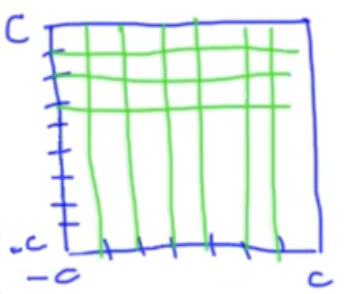
\includegraphics[width=1.5in]{./images/T46_pic.png} %таймкод: 1:50:08

        Cторона маленького кубика $= \frac{2c}{n} \Longrightarrow$ его главная диагональ $= \sqrt{d} \cdot \frac{2c}{n} < \varepsilon$

        диагональ $< \varepsilon \Longrightarrow$ расстояние между любыми двумя точками кубика $< \varepsilon$

        Итого, мы нарезали множество (большой куб) на маленькие кубики, таким образом, что в каждом кубике расстояние между двумя любыми точками $< \varepsilon$,
        таких кубиков у нас конечное число, а дальше давайте выбирать "представителей":

        Если какой-то кубик вообще не пересекаетснея с $A$, то ничего брать не будем. А если пересекается, возьмём одну точку из пересечения.

        Это будет конечное множество, более того, это $\varepsilon$-сеть.
    \end{enumerate}
\end{proof}


\begin{theorem-non}
    Хаусдорфа.

    \begin{enumerate}
        \item Компактное множество вполне ограничено.
        \item $X$ --- полное пространство, то замкнутое вполне ограниченное множество компактно.
    \end{enumerate}

    \begin{proof} \quad  

        \begin{enumerate}
            \item Берём $\varepsilon > 0$  и $K \subset \bigcup\limits_{x \in K}B_{\varepsilon}(x)$ и выберем из него конечное подпокрытие:
            
            $K \subset \bigcup\limits_{j = 1}^n B_{\varepsilon}(x_j)$. Тогда $x_1, x_2, \dots, x_n$ конечная $\varepsilon$-сеть.

            \item 
            Будем проверять секвенциальную компактность.
            
            Возьмём последовательность $x_1, x_2, \dots \in K$.

            Рассмотрим конечную $1$-сеть.
            В каком-то шарике есть бесконечное количество $x$-ов, выкинем всё лишнее, оставим только их.
            
            Рассмотрим конечную $\frac{1}{2}$-сеть, в каком-то из шариков есть бесконечное количество оставшихся $x$-ов, выкинем всё лишнее, оставим только их.

            Рассмотрим конечную $\frac{1}{3}$-сеть, в каком-то из шариков есть бесконечное количество оставшихся $x$-ов, выкинем всё лишнее, оставим только их.

            $\dots$

            $x_{11}, x_{12}, x_{13}, \dots $ в шарике $B_1(a_1)$ \\
            $x_{21}, x_{22}, x_{23}, \dots $ в шарике $B_{\frac{1}{2}}(a_2)$ \\
            $x_{31}, x_{32}, x_{33}, \dots $ в шарике $B_{\frac{1}{3}}(a_3)$  \\
            $\dots$

            (Следующая строчка подпоследовательность предыдущей)

            Возьмём $x_{11}, x_{22}, x_{33}, \dots$ --- $x_{nn}$ подпоследовательность исходной последовательности.

            $x_{nn}$ при $n \geqslant k$ --- подпоследовательность $x_{kn}$, т.е. лежит в $B_{1/k}(a_k)$

            $x_{nn} \in B_{1/k}(a_k)$ при $n \geqslant k \Longrightarrow \rho(x_{nn}, x_{mm}) \leqslant \rho(x_{nn}, a_k) + \rho(x_{mm}, a_k) < \frac{2}{k}$ при $n,m \geqslant k$

            $\Longrightarrow x_{nn}$ --- фундаментальная последовательность $\Longrightarrow$ существует $\lim{x_{nn}}= b$, т.к. $K$ --- замкнуто $b \in K \Longrightarrow K$ --- секвенц. компактно $\Longrightarrow K$ --- компактно.
            
            \end{enumerate}    
    \end{proof}

\end{theorem-non}

\notice Это рассуждение --- диагональный метод Кантора.

\begin{follow}
    Характеристика Компактов в $R^d$

    $K \subset R^d$ --- компакт $\Longleftrightarrow K$ --- замкнуто и ограничено.

    \begin{proof}
        "$\Longrightarrow$" верно всегда

        "$\Longleftarrow$" $K$ --- вполне ограничено $\Longrightarrow$ вполне огр. + замкнутость $\Longrightarrow$ компактность (т.к. $R^d$ --- полное пространство).
    \end{proof} 

\end{follow} 
